\begin{figure}[htp]
\begin{center}
	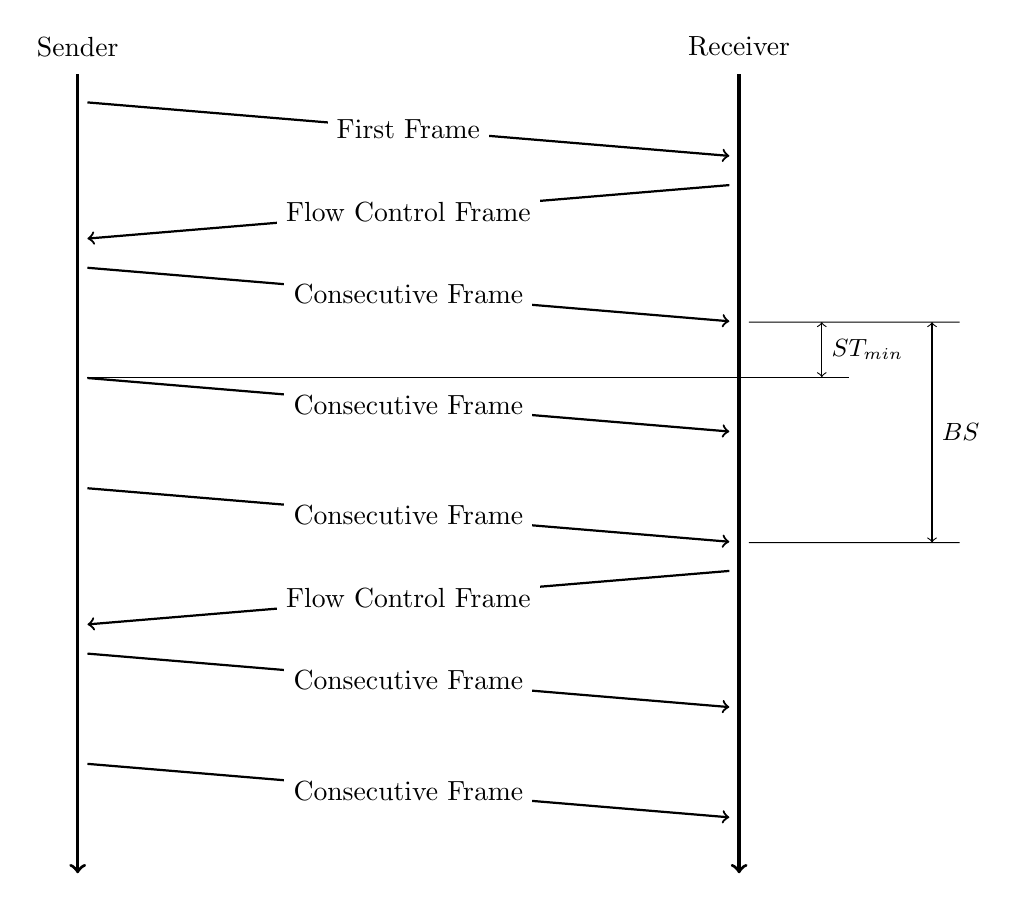
\begin{tikzpicture}[scale=0.7]
		%Sender
		\node (s_ff) at (0,14)  {};
		\node (s_fc1) at (0,11.5) {};
		\node (s_cf1) at (0,11) {};
		\node (s_cf2) at (0,9) {};
		\node (s_cf3) at (0,7) {};
		\node (s_fc2) at (0,4.5) {};
		\node (s_cf4) at (0,4) {};
		\node (s_cf5) at (0,2) {};
		
		%Receiver
		\node (r_ff) at (12,13)  {};
		\node (r_fc1) at (12,12.5) {};
		\node (r_cf1) at (12,10) {};
		\node (r_cf2) at (12,8) {};
		\node (r_cf3) at (12,6) {};
		\node (r_fc2) at (12,5.5) {};
		\node (r_cf4) at (12,3) {};
		\node (r_cf5) at (12,1) {};

		%connections
		\draw[thick, ->] (s_ff) -- node[midway, fill=white] {First Frame} (r_ff);
		\draw[thick,->] (r_fc1) -- node[midway, fill=white] {Flow Control Frame} (s_fc1);
		\draw[thick,->] (s_cf1) -- node[midway, fill=white] {Consecutive Frame} (r_cf1);
		\draw[thick,->] (s_cf2) -- node[midway, fill=white] {Consecutive Frame} (r_cf2);
		\draw[thick,->] (s_cf3) -- node[midway, fill=white] {Consecutive Frame} (r_cf3);
		\draw[thick,->] (r_fc2) -- node[midway, fill=white] {Flow Control Frame} (s_fc2);
		\draw[thick,->] (s_cf4) -- node[midway, fill=white] {Consecutive Frame} (r_cf4);
		\draw[thick,->] (s_cf5) -- node[midway, fill=white] {Consecutive Frame} (r_cf5);
		
		%stmin
		\draw (r_cf1) -- ++(4,0);
		\draw (s_cf2) -- ++(14,0);
		\draw[<->] (13.5,9) -- (13.5,10) node[midway,right]{\small $ST_{min}$};
		\draw (r_cf3) -- ++(4,0);
		\draw[<->] (15.5,6) -- (15.5,10) node[midway,right]{\small $BS$};
		
		%Flow
		\draw[very thick, ->] (0,14.5) --  (0,0);
		\node at (0,15) {Sender};
		\draw[very thick, ->] (12,14.5) -- (12,0);
		\node at (12,15) {Receiver};
		
	\end{tikzpicture}
	\caption{Example Sequence of a Segmented Packet with a BS of three}
	\label{fig:iso_tp_sequence}
\end{center}
\end{figure}